% Generated by build_report.py; shared by both documents.
\section{Phụ lục: đọc chi tiết 14 sample A/B/C}\label{sec:4}
A/B/C là các điều kiện cùng nhiệm vụ, không phải thứ tự độ khó. Mỗi ca chọn một bản ghi thật từ bộ minh họa 12 nhóm/264 chuyến; số bản ghi không phải số chuyến độc lập. \textbf{S10 chỉ có A/B} trong tài liệu; B ánh xạ mã nguồn cũ S10.C để giữ truy nguyên, không có ca C độc lập trong phạm vi hiện tại.

Chấm màu = mẫu trước bảo vệ; nét đứt = đường thật để chấm; sao đỏ = đáp án; trục thời gian tách các mẫu chồng nhau. Đối thủ chỉ nhận dữ liệu đã bảo vệ và thông tin phụ trợ được phép, không nhận các tọa độ/nhãn thật này. Bản đồ minh họa dùng nền SUMO với cùng mã kiểm tra tệp OSM; thiếu mạng gốc để xác minh trùng toàn bộ hình học. © OpenStreetMap contributors.

\subsection{S1 — suy ra vị trí tại một lần gửi}\label{sub:4.1}
Đối thủ cần suy ra tọa độ tại một lần gửi. A/B thay ràng buộc mạng đường; C thêm ngữ cảnh POI hiếm.

\noindent\begin{minipage}[t]{0.48\linewidth}\vspace{0pt}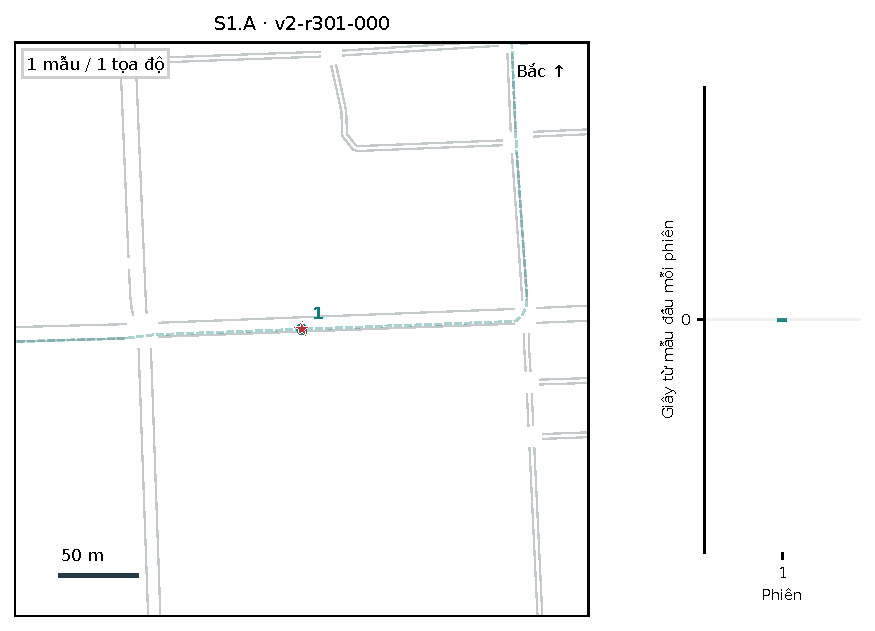
\includegraphics[width=\linewidth]{figures/case_S1_A.pdf}\end{minipage}\hfill\begin{minipage}[t]{0.49\linewidth}\vspace{0pt}\RaggedRight \textbf{S1.A / 12 bản ghi.} Một bản tin tại cạnh có $\ge$2 hướng đi tiếp hợp lệ: kiểm tra khi mạng đường còn nhiều khả năng.\par\smallskip \textbf{Bản ghi minh họa v2-r301-000.} u301\_\allowbreak{}00: 1 mẫu, chỉ số GPS FCD[333…333]\par\smallskip\textbf{Đọc sample.} Một lần lấy mẫu ở cạnh có 4 hướng đi tiếp. Sao đỏ trùng vị trí đầu vào; đối thủ phải chọn vị trí từ đầu ra đã bảo vệ, không được thấy sẵn sao này.\end{minipage}\par\vspace{3pt}
\noindent\begin{minipage}[t]{0.48\linewidth}\vspace{0pt}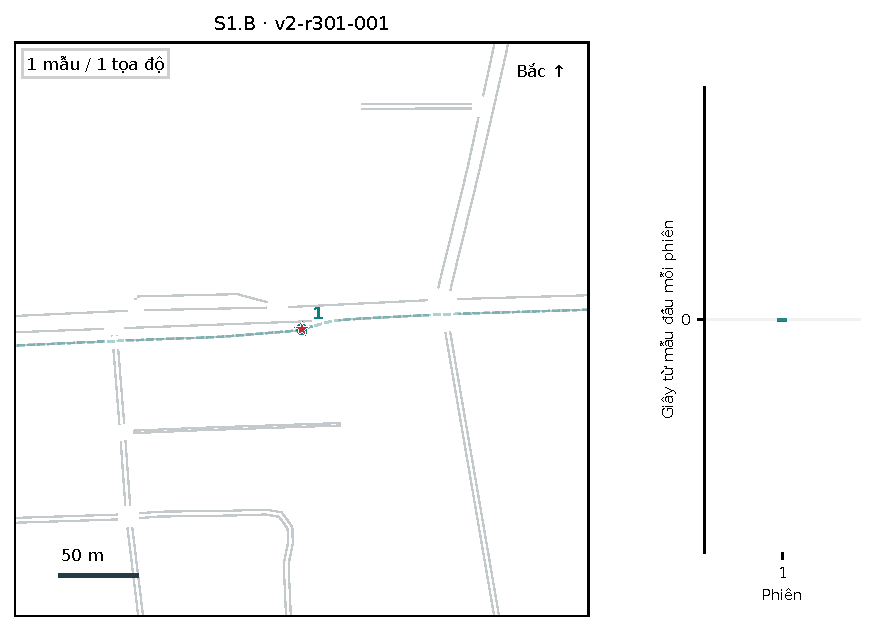
\includegraphics[width=\linewidth]{figures/case_S1_B.pdf}\end{minipage}\hfill\begin{minipage}[t]{0.49\linewidth}\vspace{0pt}\RaggedRight \textbf{S1.B / 12 bản ghi.} Một bản tin tại cạnh chỉ có 1 hướng đi tiếp: bản đồ tự loại bớt khả năng.\par\smallskip \textbf{Bản ghi minh họa v2-r301-001.} u301\_\allowbreak{}00: 1 mẫu, chỉ số GPS FCD[241…241]\par\smallskip\textbf{Đọc sample.} Vẫn chỉ một lần lấy mẫu, nhưng cạnh chỉ có một hướng đi tiếp. Bản đồ có thể loại bớt khả năng so với A; cần đo lợi thế này bằng đối thủ thực tế.\end{minipage}\par\vspace{3pt}
\noindent\begin{minipage}[t]{0.48\linewidth}\vspace{0pt}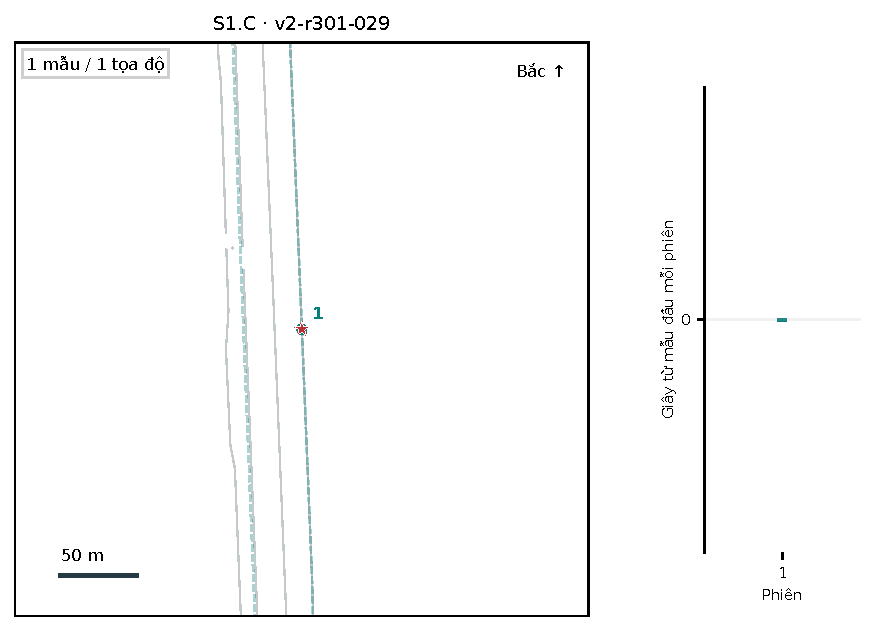
\includegraphics[width=\linewidth]{figures/case_S1_C.pdf}\end{minipage}\hfill\begin{minipage}[t]{0.49\linewidth}\vspace{0pt}\RaggedRight \textbf{S1.C / 12 bản ghi.} Cách POI $\le$150 m; loại POI chiếm $\le$5\% danh mục công khai. Hiếm theo loại địa điểm, không phải theo tần suất ghé thăm.\par\smallskip \textbf{Bản ghi minh họa v2-r301-029.} u301\_\allowbreak{}13: 1 mẫu, chỉ số GPS FCD[695…695]\par\smallskip\textbf{Đọc sample.} Điểm lấy mẫu cách POI pharmacy 12,03 m; loại này chiếm 3,11\% danh mục. Ngữ cảnh địa điểm hiếm là dấu hiệu bổ sung, không phải chuỗi di chuyển.\end{minipage}\par\vspace{3pt}

\clearpage
\subsection{S2 — suy ra nơi dừng qua nhiều lần gửi}\label{sub:4.2}
Đối thủ cần suy ra tọa độ nơi dừng. A/B thay thời lượng và nhịp quan sát; C kiểm tra rời đi rồi quay lại.

\noindent\begin{minipage}[t]{0.48\linewidth}\vspace{0pt}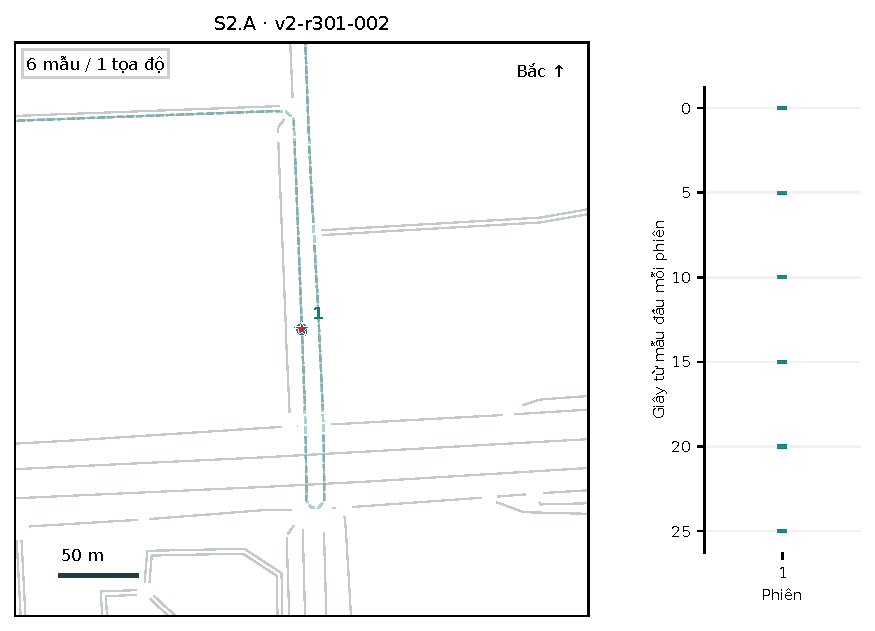
\includegraphics[width=\linewidth]{figures/case_S2_A.pdf}\end{minipage}\hfill\begin{minipage}[t]{0.49\linewidth}\vspace{0pt}\RaggedRight \textbf{S2.A / 12 bản ghi.} Dừng có chủ đích $\ge$20 giây; lấy truy vấn mỗi 5 giây.\par\smallskip \textbf{Bản ghi minh họa v2-r301-002.} u301\_\allowbreak{}05: 6 mẫu, chỉ số GPS FCD[54…79]\par\smallskip\textbf{Đọc sample.} 6 mẫu cùng một tọa độ, cách nhau 5 giây; đoạn dừng thật dài 29 giây. Sáu vạch thời gian bị chồng thành một chấm trên map.\end{minipage}\par\vspace{3pt}
\noindent\begin{minipage}[t]{0.48\linewidth}\vspace{0pt}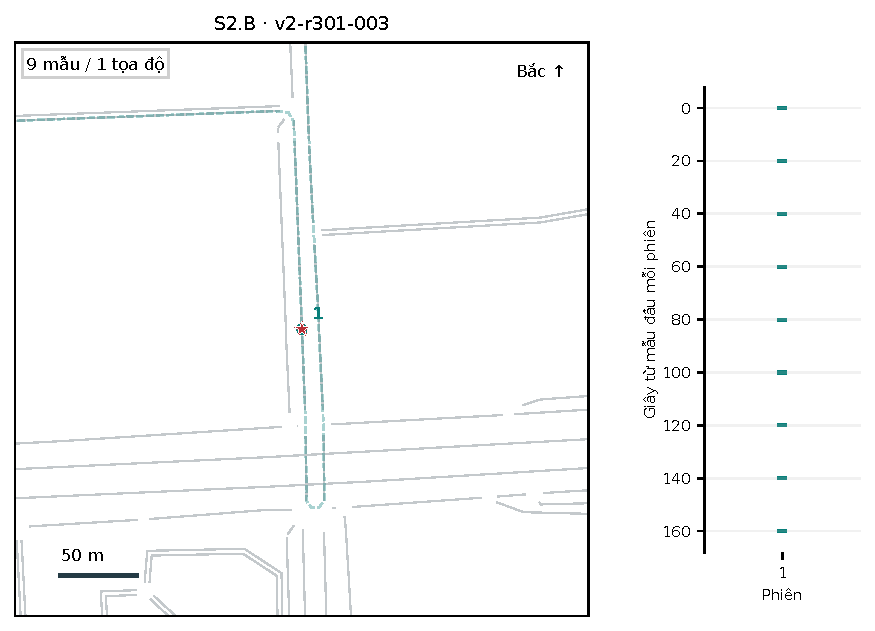
\includegraphics[width=\linewidth]{figures/case_S2_B.pdf}\end{minipage}\hfill\begin{minipage}[t]{0.49\linewidth}\vspace{0pt}\RaggedRight \textbf{S2.B / 12 bản ghi.} Dừng $\ge$120 giây; lấy truy vấn mỗi 20 giây.\par\smallskip \textbf{Bản ghi minh họa v2-r301-003.} u301\_\allowbreak{}06: 9 mẫu, chỉ số GPS FCD[59…219]\par\smallskip\textbf{Đọc sample.} 9 mẫu cùng một tọa độ, cách nhau 20 giây; đoạn dừng dài 179 giây. Đối thủ có cửa sổ dài hơn để kết hợp bằng chứng, không chỉ một bản tin.\end{minipage}\par\vspace{3pt}
\noindent\begin{minipage}[t]{0.48\linewidth}\vspace{0pt}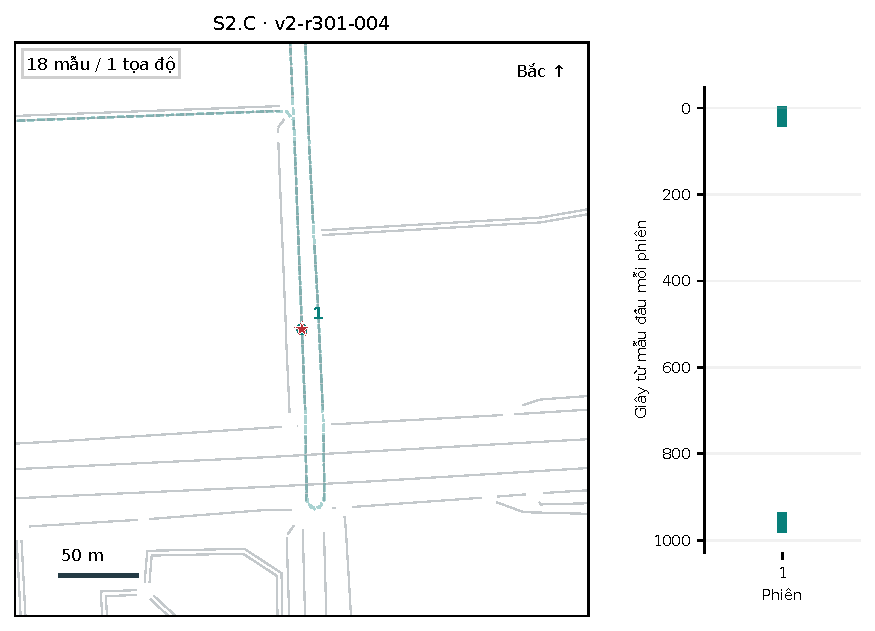
\includegraphics[width=\linewidth]{figures/case_S2_C.pdf}\end{minipage}\hfill\begin{minipage}[t]{0.49\linewidth}\vspace{0pt}\RaggedRight \textbf{S2.C / 12 bản ghi.} Hai lần dừng trên cùng làn, mỗi lần $\ge$20 giây; ở giữa thực sự di chuyển.\par\smallskip \textbf{Bản ghi minh họa v2-r301-004.} u301\_\allowbreak{}07: 18 mẫu, chỉ số GPS FCD[214…1193]\par\smallskip\textbf{Đọc sample.} 18 mẫu chia hai đợt, mỗi đợt 9 mẫu. Hai lần dừng dài 44 giây tại cùng tọa độ; khoảng trống giữa hai cụm thời gian là lúc xe rời đi rồi quay lại.\end{minipage}\par\vspace{3pt}

\clearpage
\subsection{S3 — tái dựng đoạn đường đã đi}\label{sub:4.3}
Đối thủ cần tái dựng các vị trí của đoạn đã đi. A là chuỗi đều; B ít nhánh; C quan sát thưa.

\noindent\begin{minipage}[t]{0.48\linewidth}\vspace{0pt}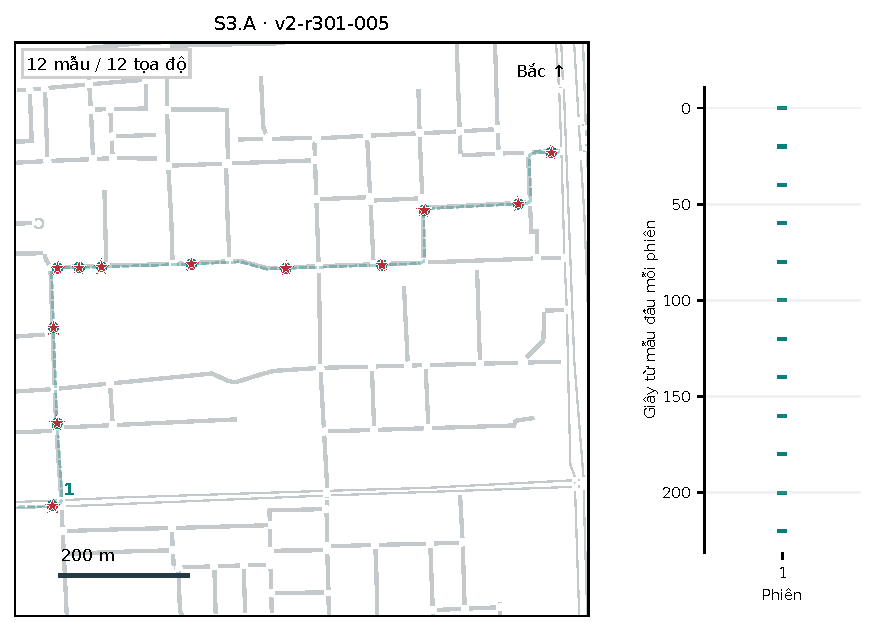
\includegraphics[width=\linewidth]{figures/case_S3_A.pdf}\end{minipage}\hfill\begin{minipage}[t]{0.49\linewidth}\vspace{0pt}\RaggedRight \textbf{S3.A / 12 bản ghi.} Đoạn di chuyển $\ge$60 giây qua $\ge$3 cạnh; gửi mỗi 20 giây.\par\smallskip \textbf{Bản ghi minh họa v2-r301-005.} u301\_\allowbreak{}00: 12 mẫu, chỉ số GPS FCD[361…581]\par\smallskip\textbf{Đọc sample.} 12 mẫu của u301\_\allowbreak{}00 cách nhau 20 giây. Chuỗi điểm cung cấp nhiều ràng buộc để nối tuyến; nét đứt là đường thật chỉ dùng chấm.\end{minipage}\par\vspace{3pt}
\noindent\begin{minipage}[t]{0.48\linewidth}\vspace{0pt}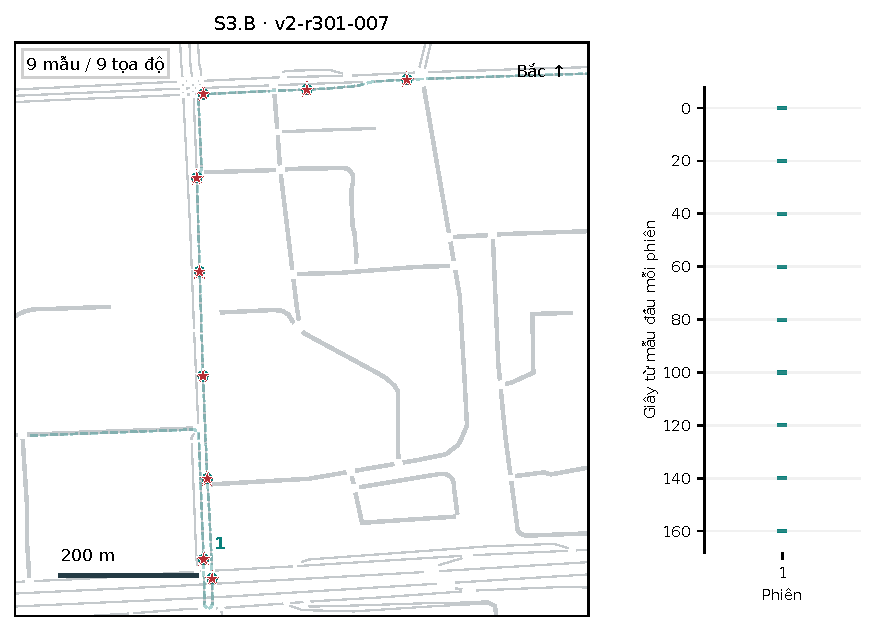
\includegraphics[width=\linewidth]{figures/case_S3_B.pdf}\end{minipage}\hfill\begin{minipage}[t]{0.49\linewidth}\vspace{0pt}\RaggedRight \textbf{S3.B / 11 bản ghi.} Ít nhất một nửa số cạnh được lấy mẫu chỉ có một hướng đi tiếp: hành lang ít lựa chọn.\par\smallskip \textbf{Bản ghi minh họa v2-r301-007.} u301\_\allowbreak{}00: 9 mẫu, chỉ số GPS FCD[91…251]\par\smallskip\textbf{Đọc sample.} 9 mẫu; 55,6\% cạnh được lấy mẫu chỉ có một hướng đi tiếp. Đường ít nhánh có thể khiến chuỗi dễ suy hơn dù từng vị trí được làm mờ.\end{minipage}\par\vspace{3pt}
\noindent\begin{minipage}[t]{0.48\linewidth}\vspace{0pt}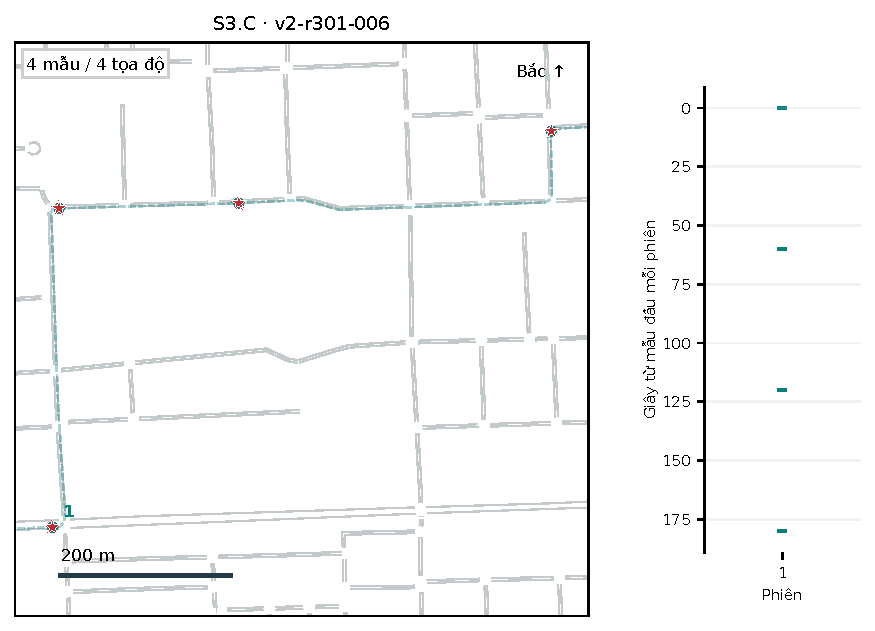
\includegraphics[width=\linewidth]{figures/case_S3_C.pdf}\end{minipage}\hfill\begin{minipage}[t]{0.49\linewidth}\vspace{0pt}\RaggedRight \textbf{S3.C / 12 bản ghi.} Lấy mẫu đoạn di chuyển thưa hơn, mỗi 60 giây.\par\smallskip \textbf{Bản ghi minh họa v2-r301-006.} u301\_\allowbreak{}00: 4 mẫu, chỉ số GPS FCD[361…541]\par\smallskip\textbf{Đọc sample.} 4 mẫu của cùng đoạn trong A, cách nhau 60 giây. Khoảng trống lớn hơn nhưng đối thủ vẫn có thể dùng mạng đường để nối các khả năng.\end{minipage}\par\vspace{3pt}

\clearpage
\subsection{S9 — suy ra điểm xuất phát bị che}\label{sub:4.4}
Đối thủ cần suy điểm đầu bị giấu. A suy ngược một chuyến; B phân biệt hai nguồn nhập tuyến; C kết hợp chuyến lặp.

\noindent\begin{minipage}[t]{0.48\linewidth}\vspace{0pt}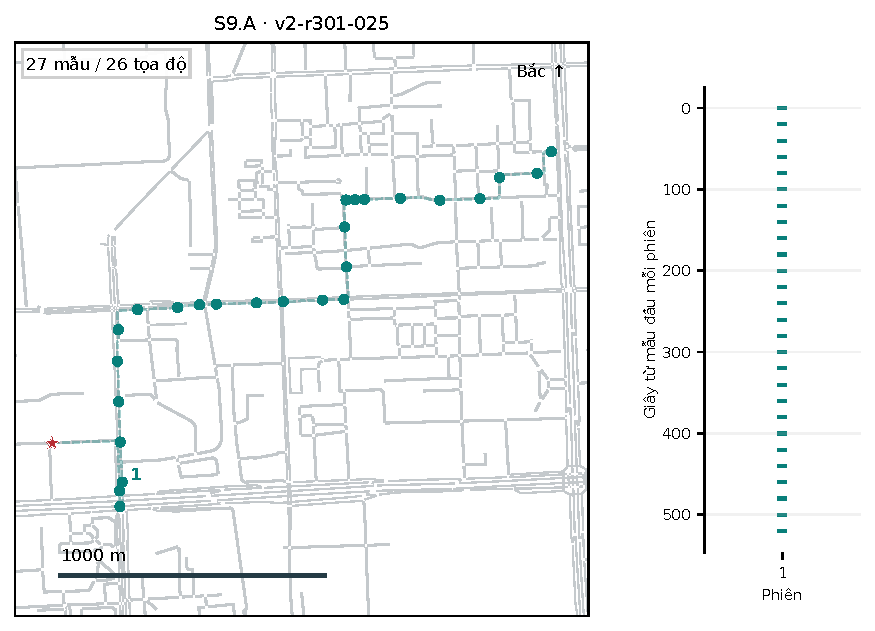
\includegraphics[width=\linewidth]{figures/case_S9_A.pdf}\end{minipage}\hfill\begin{minipage}[t]{0.49\linewidth}\vspace{0pt}\RaggedRight \textbf{S9.A / 12 bản ghi.} Cạnh xuất phát chỉ một lối ra. Che 60 giây đầu, lấy phần còn lại mỗi 20 giây.\par\smallskip \textbf{Bản ghi minh họa v2-r301-025.} u301\_\allowbreak{}00: 27 mẫu, chỉ số GPS FCD[60…580]\par\smallskip\textbf{Đọc sample.} Sao là FCD[0]; cửa sổ bắt đầu ở FCD[60] sau khi che 60 giây. Chỉ một lối ra có thể giúp suy ngược nguồn xuất phát từ phần còn công bố.\end{minipage}\par\vspace{3pt}
\noindent\begin{minipage}[t]{0.48\linewidth}\vspace{0pt}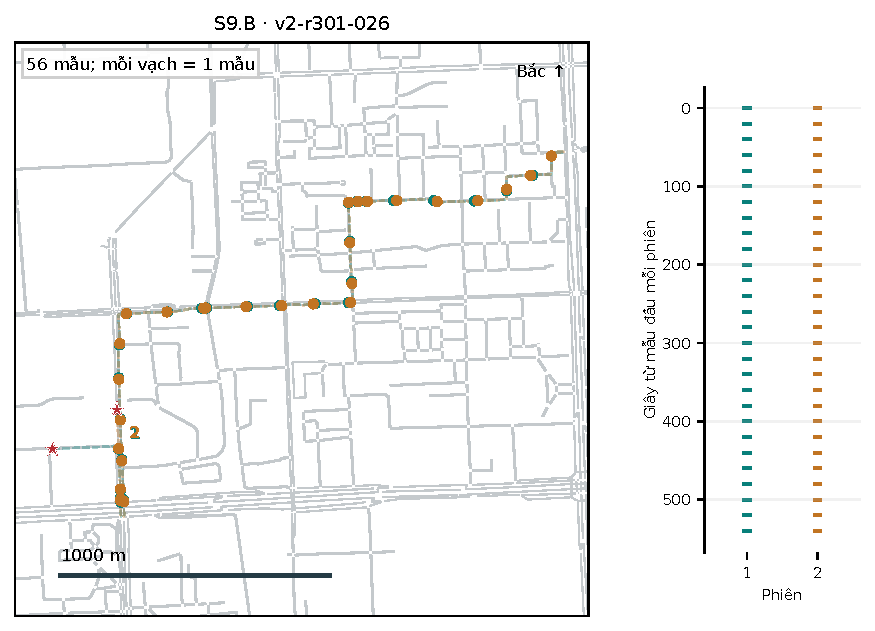
\includegraphics[width=\linewidth]{figures/case_S9_B.pdf}\end{minipage}\hfill\begin{minipage}[t]{0.49\linewidth}\vspace{0pt}\RaggedRight \textbf{S9.B / 11 bản ghi.} Hai chuyến khác điểm đầu nhưng nhập một đoạn chung; chỉ cấp từ chỗ nhập tuyến.\par\smallskip \textbf{Bản ghi minh họa v2-r301-026.} u301\_\allowbreak{}00: 28 mẫu, chỉ số GPS FCD[34…574]; u301\_\allowbreak{}04: 28 mẫu, chỉ số GPS FCD[19…559]\par\smallskip\textbf{Đọc sample.} Hai điểm đầu cách 281,76 m rồi nhập tuyến. Chỉ cấp dữ liệu sau nhập; hai sao là hai đáp án bị giấu mà đối thủ phải phân biệt.\end{minipage}\par\vspace{3pt}
\noindent\begin{minipage}[t]{0.48\linewidth}\vspace{0pt}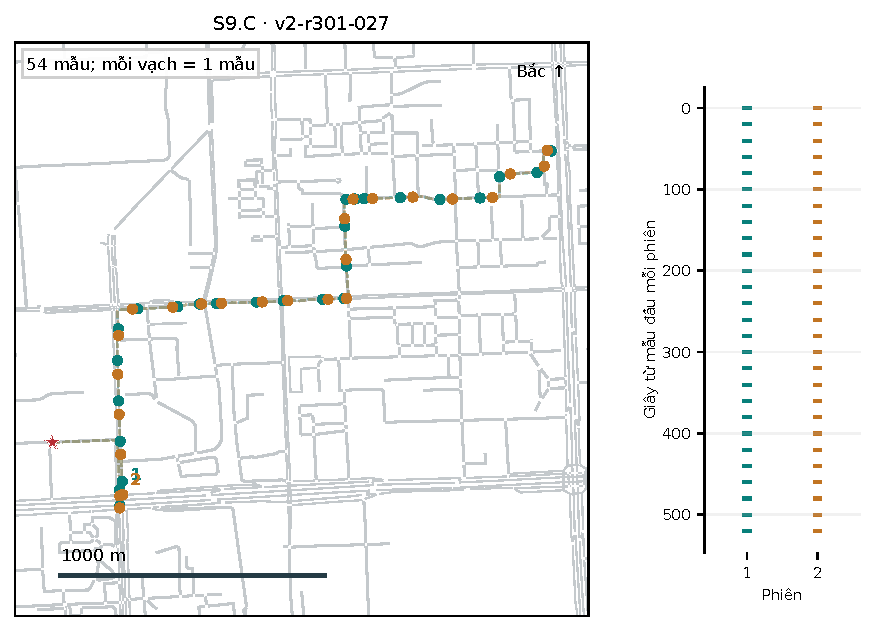
\includegraphics[width=\linewidth]{figures/case_S9_C.pdf}\end{minipage}\hfill\begin{minipage}[t]{0.49\linewidth}\vspace{0pt}\RaggedRight \textbf{S9.C / 12 bản ghi.} Nhiều chuyến có cùng điểm xuất phát dự kiến; che 60 giây đầu từng chuyến.\par\smallskip \textbf{Bản ghi minh họa v2-r301-027.} u301\_\allowbreak{}00: 27 mẫu, chỉ số GPS FCD[60…580]; u301\_\allowbreak{}09: 27 mẫu, chỉ số GPS FCD[60…580]\par\smallskip\textbf{Đọc sample.} u301\_\allowbreak{}00/u301\_\allowbreak{}09 lặp cùng điểm đầu dự kiến; mỗi phiên che 60 giây đầu. Nhiều cửa sổ có thể bổ sung bằng chứng về cùng nguồn xuất phát.\end{minipage}\par\vspace{3pt}

\clearpage
\subsection{S10 — suy ra điểm kết thúc bị che}\label{sub:4.5}
Đối thủ cần suy điểm cuối của chuyến đã hoàn tất. A dùng một chuyến; B kết hợp nhiều chuyến cùng đích. Đây khác dự đoán đích tương lai ở S6.

\noindent\begin{minipage}[t]{0.58\linewidth}\vspace{0pt}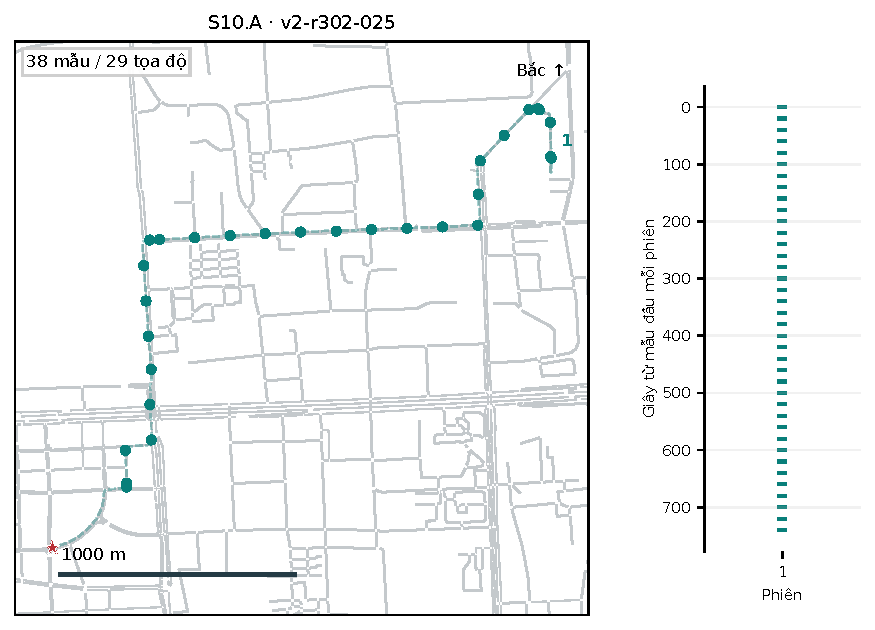
\includegraphics[width=\linewidth]{figures/case_S10_A.pdf}\end{minipage}\hfill\begin{minipage}[t]{0.39\linewidth}\vspace{0pt}\RaggedRight \textbf{S10.A / 11 bản ghi.} Cạnh kết thúc chỉ một lối vào. Che 60 giây cuối của chuyến đã hoàn tất.\par\smallskip \textbf{Bản ghi minh họa v2-r302-025.} u302\_\allowbreak{}08: 38 mẫu, chỉ số GPS FCD[0…740]\par\smallskip\textbf{Đọc sample.} Sao là FCD cuối [817] của u302\_\allowbreak{}08; che 60 giây cuối. Đường chỉ một lối vào có thể giúp suy đoạn kết thúc từ phần trước còn thấy.\end{minipage}\par\vspace{3pt}
\noindent\begin{minipage}[t]{0.58\linewidth}\vspace{0pt}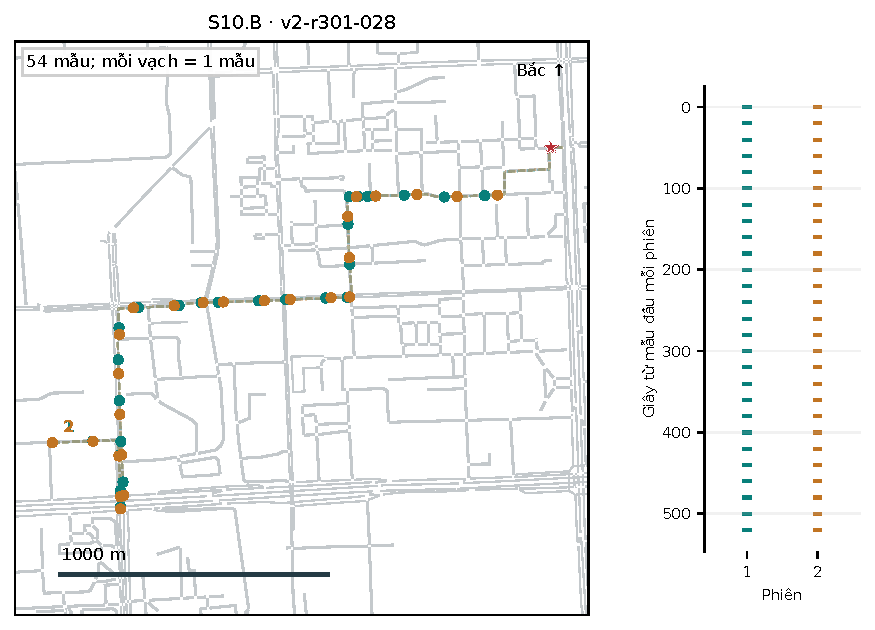
\includegraphics[width=\linewidth]{figures/case_S10_B.pdf}\end{minipage}\hfill\begin{minipage}[t]{0.39\linewidth}\vspace{0pt}\RaggedRight \textbf{S10.B / 12 bản ghi.} Nhiều chuyến cùng điểm kết thúc dự kiến; che 60 giây cuối từng chuyến.\par\smallskip \textbf{Bản ghi minh họa v2-r301-028.} u301\_\allowbreak{}00: 27 mẫu, chỉ số GPS FCD[0…520]; u301\_\allowbreak{}09: 27 mẫu, chỉ số GPS FCD[0…520]\par\smallskip\textbf{Đọc sample.} u301\_\allowbreak{}00/u301\_\allowbreak{}09 lặp cùng đích dự kiến và cùng che 60 giây cuối. Đối thủ có thể kết hợp nhiều phiên để khoanh đích, chưa đủ gọi đó là nơi làm việc.\end{minipage}\par\vspace{3pt}
S9/S10 chấm tọa độ đầu/cuối; chưa gán nhãn nhà/nơi làm việc. Xem bản đồ phóng to của 29 ca của khung đầy đủ ở sample\_\allowbreak{}maps.html; tọa độ và bản ghi ở data\_\allowbreak{}samples.json, số đếm ở scenario\_\allowbreak{}inventory.csv.


\clearpage
